\begin{titlepage}
\begin{otherlanguage}{ngerman}
\onehalfspacing
\pagenumbering{Roman}
\newgeometry{top=2.28cm,bottom=2.28cm,left=\SeitenrandLinks,right=\SeitenrandLinks}
\begin{center}
\begin{figure}[t]
\makebox[\textwidth]{
\includegraphics[scale=0.15]{titlepage/figures/logo.pdf}}
\end{figure}
{\Large \textbf{Monotonie und Monotoniesensitivität als Desiderata für Maße der Bedarfsgerechtigkeit}}\\[0.5cm]
{\large \textbf{Zu zwei Aspekten der Grundlegung empirisch informierter Maße der Bedarfsgerechtigkeit zwischen normativer Theorie, formaler Modellierung und empirischer Sozialforschung}}\\[2cm]
\makebox[\textwidth]{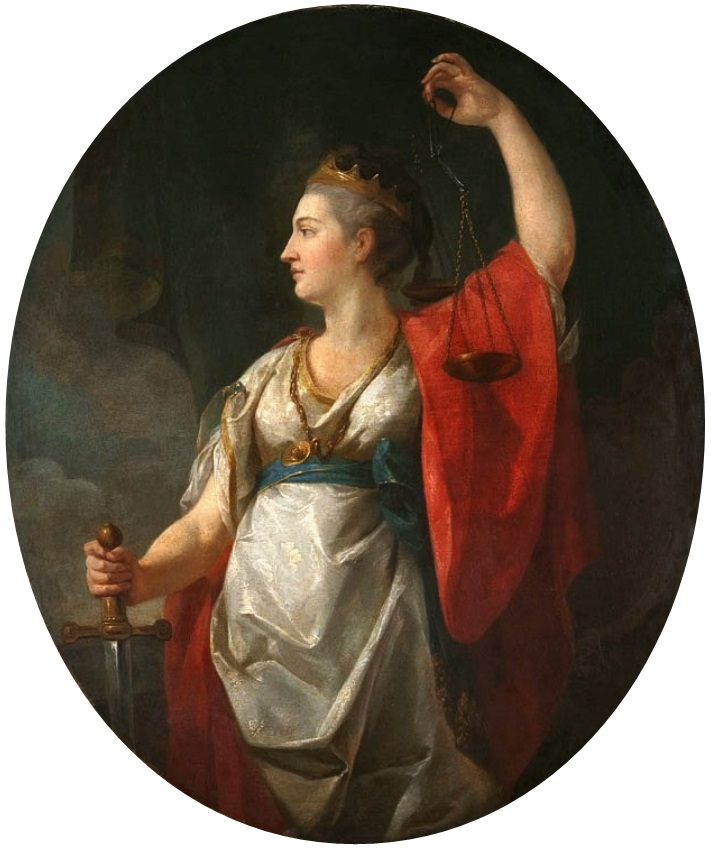
\includegraphics[scale=0.45]{titlepage/figures/bacciarelli_themis.jpg}}\\[1cm]
{\large \textbf{\DeinName}}\\[0.5cm]
Januar 2018\\[0.5cm]
Titelabbildung:\\
Marcello Bacciarelli -- Themis
\end{center}
\end{otherlanguage}
\end{titlepage}
\restoregeometry
\MSonehalfspacing
\cleardoublepage
\setcounter{savepage}{\arabic{page}}
\pagenumbering{arabic}